\documentclass{ctexbeamer}        % 文档类beamer的汉化版本

\usefonttheme{serif}              % 使用衬线字体
\usefonttheme{professionalfonts}  % 数学公式字体

\usepackage{mathtools}
\usepackage{hyperref}
\hypersetup{pdfpagemode=FullScreen}  %用PDF 阅读器打开时自动全屏显示

\usepackage[UTF8]{ctex}       %中文
\usepackage{microtype}        %排版相关
\usepackage[american]{babel}  %排版相关
\usepackage{amsmath}          %数学公式
\usepackage{amssymb}          %数学公式
\usepackage{url}
\usepackage{tikz}
%\usepackage{gnuplot-lua-tikz}
\usepackage{graphicx}
\usetikzlibrary{calc,positioning, shapes.geometric}

%% --> 配置中英文字体
% \usepackage{fontspec}
% \setmainfont{Liberation Serif}
% \setsansfont{DejaVu Sans}
% \setmonofont{Cousine}
% \usepackage{xeCJK}
% \setCJKmainfont[BoldFont=Noto Sans SC]{Noto Serif SC}
% \setCJKsansfont{Noto Sans SC}
% \setCJKmonofont{WenQuanYi Micro Hei Mono}

%% --> 主题和色彩风格
\usetheme{Frankfurt}       %主题和色彩可以自由搭配
\usecolortheme{orchid}     %主题和色彩的样式可参见网页 https://mpetroff.net/files/beamer-theme-matrix/


\begin{document}
	
	%% --> 导言页
	%
	\title{一维非线性方程的求解}
	\author{Janice\_zh}
	\institute{浙江大学}
	\date{\today}
	\frame{\titlepage}
	
	%% --> 目录结构
	%
	\begin{frame}{目录}         %自动生成目录
		\tableofcontents[hideallsubsections]
	\end{frame}
	
	%% --> 正式内容开始
	%
	\section{引言}    % 第 1 节
	
	%% 每一节开头显示目录,并高亮当前节的主题
	%\AtBeginSection[]{\frame{\tableofcontents[currentsection,hideallsubsections]}}
	
	%% --> 第 1 帧
	\begin{frame}{引言}
		\textbf{一维非线性方程 : $f(x)=0$}\\ \par
		
		· 对于一维低阶线性方程,由公式法或其他方法易得方程的根\par
		
		· 阶数较高时,很难直接利用公式法求解,考虑迭代法
	\end{frame}
	
	\section{迭代法求解}
	%% --> 第 2 帧
	\begin{frame}{解法分类}
		下对求解一维非线性方程的迭代法进行分类:
		$$
		\begin{cases}
		root  braketing 
		\begin{cases}bisection\\falsepos\\Brent
		\end{cases}
		\\
		root  polishing 
		
		\begin{cases}
		Newton\\
		secant \\
		steffenson 
		\end{cases}
		\end{cases}
		$$
	\end{frame}
	\section{算法实现举例}
	\begin{frame}{算法实现}
		\textbf{二分法:} \\给定可能解区间,每次取中点二分进行迭代。是最简单的一种迭代方式,线性收敛。同时要求给定区间端点的函数值异号,且不能处理偶数重根的情况。\\
		\textbf{牛顿法:} \\不断迭代近似解,切线与x轴的交点迭代成为新的近似解。单根二次收敛,复根线性收敛。求解效率与准确度比较依赖初始近似解的选取。\\
		\textbf{secant法:}\\牛顿法的简化,从第二步开始用数值估计替代导数。多重根线性收敛。适合在根附近导数无明显变化的函数方程,依赖原方程的特点与初始近似解的选取。
	\end{frame}
	\begin{frame}{收敛性比较}
		· 分别用二分法,牛顿法,secant法求解$x^2-5=0$。\\ 
		· 一般来讲,牛顿法与secant法相对于二分法,收敛性更强,收敛速度更快,所得解精度更高
	\end{frame}
	\section{数值算例}    % 第 2 节
	\begin{frame}{Examples}
		下用牛顿法实现不同式子的求解。求解时应选取合适的初始近似解。
		
		\paragraph{Example1:}求解$2x^2+4x-3=0$
		\begin{figure}[ht]
			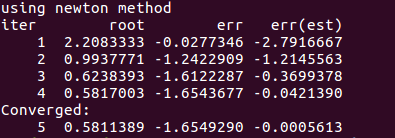
\includegraphics[width=1\linewidth]{n2.png}
		\end{figure}
		\paragraph{Example2:}求解$x^2+5=0$ \\
		(注:选取不当的初始估计解会造成无法求解)
		
	\end{frame}
	%% --> 第 3 帧
	\section{总结}
	\begin{frame}{总结}
		利用二分法、牛顿法、secant法等我们可以实现对一维非线性方程的求解。在求解过程中需注意选取合适的解区间或初始近似解。同时,给定同一方程时,不同的方法对应不同的迭代速度,我们可以结合给定方程的性质,选取合适的方法进行求解,从而获得更高的效率与更精确的结果。
	\end{frame}
	
	\begin{frame}{致谢}    %%谢谢
		%	\vspace{0.4\textheight}
		\begin{center}
			\Huge\color{blue}\bfseries Thanks!
		\end{center}
	\end{frame}
	
\end{document}